\documentclass{standalone}
\usepackage{tikz}
\usetikzlibrary{patterns, positioning}


\begin{document}
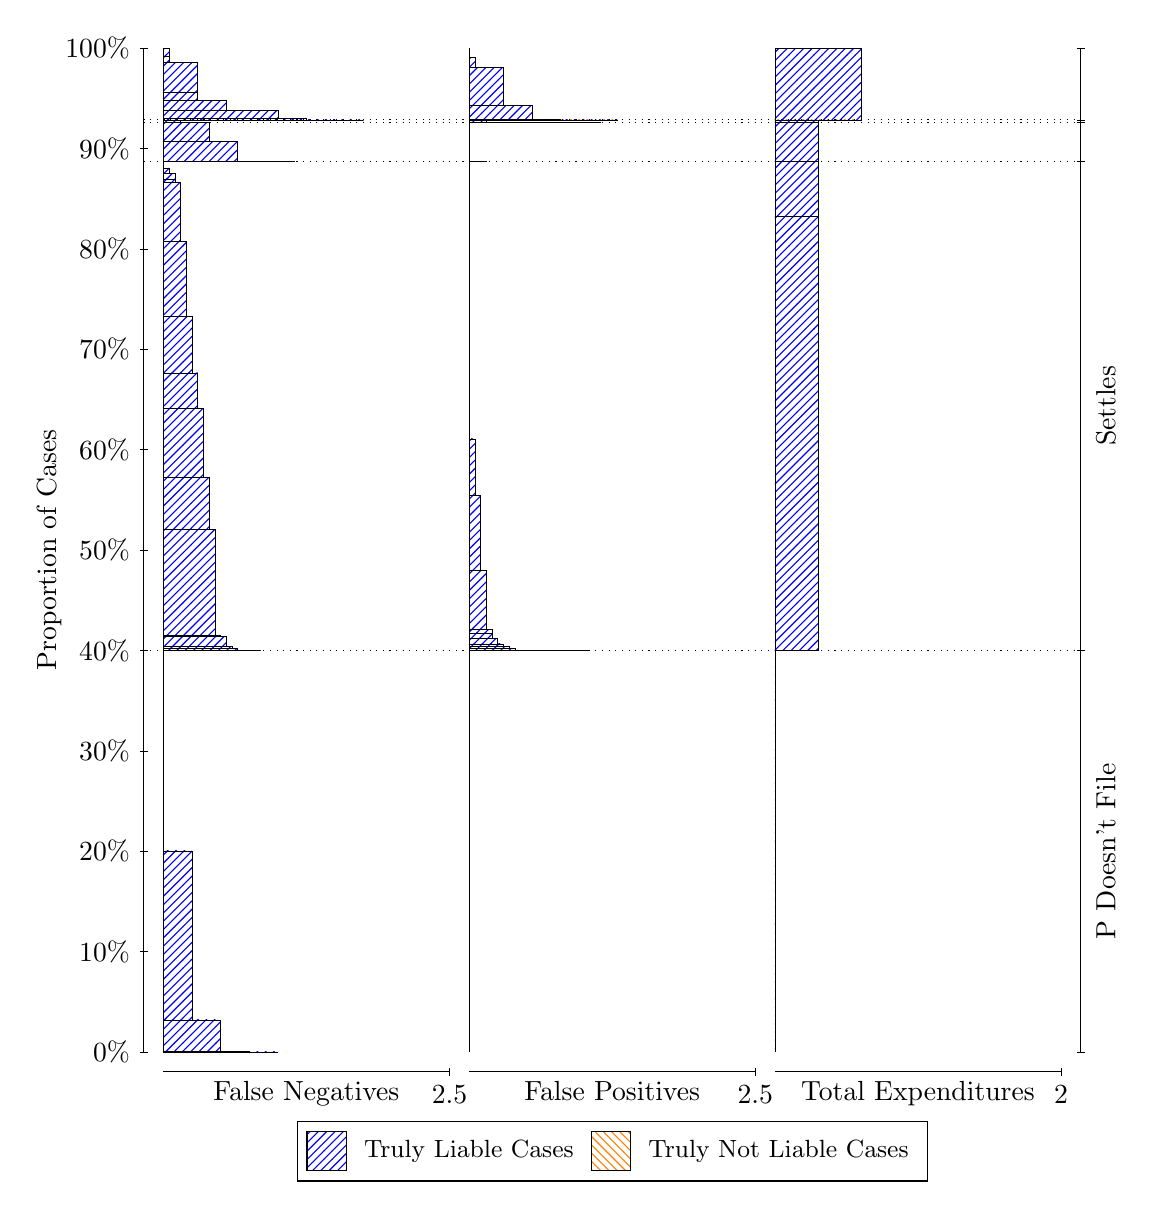
\begin{tikzpicture}
\draw[black, very thin] (1.5,1.75) -- (1.5,14.5);
\node[rotate=90, text=black, anchor=center] at (0.3, 8.125) {Proportion of Cases};
\draw[black, very thin] (1.45,1.75) -- (1.55,1.75);
\node[text=black, anchor=east] at (1.45, 1.75) {0\%};
\draw[black, very thin] (1.45,3.025) -- (1.55,3.025);
\node[text=black, anchor=east] at (1.45, 3.025) {10\%};
\draw[black, very thin] (1.45,4.3) -- (1.55,4.3);
\node[text=black, anchor=east] at (1.45, 4.3) {20\%};
\draw[black, very thin] (1.45,5.575) -- (1.55,5.575);
\node[text=black, anchor=east] at (1.45, 5.575) {30\%};
\draw[black, very thin] (1.45,6.85) -- (1.55,6.85);
\node[text=black, anchor=east] at (1.45, 6.85) {40\%};
\draw[black, very thin] (1.45,8.125) -- (1.55,8.125);
\node[text=black, anchor=east] at (1.45, 8.125) {50\%};
\draw[black, very thin] (1.45,9.4) -- (1.55,9.4);
\node[text=black, anchor=east] at (1.45, 9.4) {60\%};
\draw[black, very thin] (1.45,10.675) -- (1.55,10.675);
\node[text=black, anchor=east] at (1.45, 10.675) {70\%};
\draw[black, very thin] (1.45,11.95) -- (1.55,11.95);
\node[text=black, anchor=east] at (1.45, 11.95) {80\%};
\draw[black, very thin] (1.45,13.225) -- (1.55,13.225);
\node[text=black, anchor=east] at (1.45, 13.225) {90\%};
\draw[black, very thin] (1.45,14.5) -- (1.55,14.5);
\node[text=black, anchor=east] at (1.45, 14.5) {100\%};

\draw[black, very thin] (13.4,1.75) -- (13.4,14.5);
\draw[black, very thin] (13.35,1.75) -- (13.45,1.75);
\node[anchor=west] at (13.35, 1.75) {};
\draw[black, very thin] (13.35,6.8489) -- (13.45,6.8489);
\node[anchor=west] at (13.35, 6.8489) {};
\draw[black, very thin] (13.35,13.061) -- (13.45,13.061);
\node[anchor=west] at (13.35, 13.061) {};
\draw[black, very thin] (13.35,13.557) -- (13.45,13.557);
\node[anchor=west] at (13.35, 13.557) {};
\draw[black, very thin] (13.35,13.588) -- (13.45,13.588);
\node[anchor=west] at (13.35, 13.588) {};
\draw[black, very thin] (13.35,14.5) -- (13.45,14.5);
\node[anchor=west] at (13.35, 14.5) {};

\draw[black, very thin, pattern color=blue, pattern=north east lines] (1.75,1.75) rectangle (3.2033,1.75);
\draw[black, very thin, pattern color=blue, pattern=north east lines] (1.75,1.75) rectangle (2.84,1.7534);
\draw[black, very thin, pattern color=blue, pattern=north east lines] (1.75,1.7534) rectangle (2.4767,2.158);
\draw[black, very thin, pattern color=blue, pattern=north east lines] (1.75,2.158) rectangle (2.1133,4.3029);
\draw[black, very thin, pattern color=orange, pattern=north west lines] (1.75,4.3029) rectangle (1.75,4.3029);
\draw[black, very thin, pattern color=blue, pattern=north east lines] (1.75,4.3029) rectangle (1.75,6.8489);
\draw[black, very thin, pattern color=blue, pattern=north east lines] (1.75,6.8489) rectangle (2.9853,6.8489);
\draw[black, very thin, pattern color=blue, pattern=north east lines] (1.75,6.8489) rectangle (2.84,6.8489);
\draw[black, very thin, pattern color=blue, pattern=north east lines] (1.75,6.8489) rectangle (2.6947,6.8731);
\draw[black, very thin, pattern color=blue, pattern=north east lines] (1.75,6.8731) rectangle (2.622,6.9057);
\draw[black, very thin, pattern color=blue, pattern=north east lines] (1.75,6.9057) rectangle (2.5493,7.0264);
\draw[black, very thin, pattern color=blue, pattern=north east lines] (1.75,7.0264) rectangle (2.4767,7.0423);
\draw[black, very thin, pattern color=blue, pattern=north east lines] (1.75,7.0423) rectangle (2.404,8.3912);
\draw[black, very thin, pattern color=blue, pattern=north east lines] (1.75,8.3912) rectangle (2.3313,9.0504);
\draw[black, very thin, pattern color=blue, pattern=north east lines] (1.75,9.0504) rectangle (2.2587,9.9201);
\draw[black, very thin, pattern color=blue, pattern=north east lines] (1.75,9.9201) rectangle (2.186,10.373);
\draw[black, very thin, pattern color=blue, pattern=north east lines] (1.75,10.373) rectangle (2.1133,11.094);
\draw[black, very thin, pattern color=blue, pattern=north east lines] (1.75,11.094) rectangle (2.0407,12.048);
\draw[black, very thin, pattern color=blue, pattern=north east lines] (1.75,12.048) rectangle (1.968,12.791);
\draw[black, very thin, pattern color=blue, pattern=north east lines] (1.75,12.791) rectangle (1.8953,12.838);
\draw[black, very thin, pattern color=blue, pattern=north east lines] (1.75,12.838) rectangle (1.8953,12.904);
\draw[black, very thin, pattern color=blue, pattern=north east lines] (1.75,12.904) rectangle (1.8227,12.978);
\draw[black, very thin, pattern color=orange, pattern=north west lines] (1.75,12.978) rectangle (1.75,12.978);
\draw[black, very thin, pattern color=blue, pattern=north east lines] (1.75,12.978) rectangle (1.75,13.061);
\draw[black, very thin, pattern color=blue, pattern=north east lines] (1.75,13.061) rectangle (3.4213,13.061);
\draw[black, very thin, pattern color=blue, pattern=north east lines] (1.75,13.061) rectangle (3.058,13.065);
\draw[black, very thin, pattern color=blue, pattern=north east lines] (1.75,13.065) rectangle (2.6947,13.319);
\draw[black, very thin, pattern color=blue, pattern=north east lines] (1.75,13.319) rectangle (2.3313,13.554);
\draw[black, very thin, pattern color=blue, pattern=north east lines] (1.75,13.554) rectangle (1.968,13.557);
\draw[black, very thin, pattern color=orange, pattern=north west lines] (1.75,13.557) rectangle (1.75,13.557);
\draw[black, very thin, pattern color=blue, pattern=north east lines] (1.75,13.557) rectangle (1.968,13.587);
\draw[black, very thin, pattern color=orange, pattern=north west lines] (1.75,13.587) rectangle (1.75,13.587);
\draw[black, very thin, pattern color=blue, pattern=north east lines] (1.75,13.587) rectangle (1.75,13.588);
\draw[black, very thin, pattern color=blue, pattern=north east lines] (1.75,13.588) rectangle (4.2933,13.588);
\draw[black, very thin, pattern color=blue, pattern=north east lines] (1.75,13.588) rectangle (3.93,13.588);
\draw[black, very thin, pattern color=blue, pattern=north east lines] (1.75,13.588) rectangle (3.5667,13.608);
\draw[black, very thin, pattern color=blue, pattern=north east lines] (1.75,13.608) rectangle (3.276,13.608);
\draw[black, very thin, pattern color=blue, pattern=north east lines] (1.75,13.608) rectangle (3.2033,13.706);
\draw[black, very thin, pattern color=blue, pattern=north east lines] (1.75,13.706) rectangle (2.9127,13.707);
\draw[black, very thin, pattern color=blue, pattern=north east lines] (1.75,13.707) rectangle (2.84,13.71);
\draw[black, very thin, pattern color=blue, pattern=north east lines] (1.75,13.71) rectangle (2.5493,13.835);
\draw[black, very thin, pattern color=blue, pattern=north east lines] (1.75,13.835) rectangle (2.4767,13.835);
\draw[black, very thin, pattern color=blue, pattern=north east lines] (1.75,13.835) rectangle (2.186,13.938);
\draw[black, very thin, pattern color=blue, pattern=north east lines] (1.75,13.938) rectangle (2.186,14.314);
\draw[black, very thin, pattern color=blue, pattern=north east lines] (1.75,14.314) rectangle (2.1133,14.314);
\draw[black, very thin, pattern color=blue, pattern=north east lines] (1.75,14.314) rectangle (1.8227,14.393);
\draw[black, very thin, pattern color=blue, pattern=north east lines] (1.75,14.393) rectangle (1.8227,14.491);
\draw[black, very thin, pattern color=orange, pattern=north west lines] (1.75,14.491) rectangle (1.75,14.491);
\draw[black, very thin, pattern color=blue, pattern=north east lines] (1.75,14.491) rectangle (1.75,14.5);
\draw[black, very thin, pattern color=orange, pattern=north west lines] (5.6333,1.75) rectangle (5.6333,1.75);
\draw[black, very thin, pattern color=blue, pattern=north east lines] (5.6333,1.75) rectangle (5.6333,6.8489);
\draw[black, very thin, pattern color=orange, pattern=north west lines] (5.6333,6.8489) rectangle (7.1593,6.8489);
\draw[black, very thin, pattern color=blue, pattern=north east lines] (5.6333,6.8489) rectangle (7.1593,6.8489);
\draw[black, very thin, pattern color=orange, pattern=north west lines] (5.6333,6.8489) rectangle (7.014,6.8489);
\draw[black, very thin, pattern color=blue, pattern=north east lines] (5.6333,6.8489) rectangle (7.014,6.8489);
\draw[black, very thin, pattern color=orange, pattern=north west lines] (5.6333,6.8489) rectangle (6.8687,6.8489);
\draw[black, very thin, pattern color=blue, pattern=north east lines] (5.6333,6.8489) rectangle (6.8687,6.8489);
\draw[black, very thin, pattern color=blue, pattern=north east lines] (5.6333,6.8489) rectangle (6.796,6.8489);
\draw[black, very thin, pattern color=orange, pattern=north west lines] (5.6333,6.8489) rectangle (6.7233,6.8489);
\draw[black, very thin, pattern color=blue, pattern=north east lines] (5.6333,6.8489) rectangle (6.7233,6.8489);
\draw[black, very thin, pattern color=blue, pattern=north east lines] (5.6333,6.8489) rectangle (6.6507,6.8489);
\draw[black, very thin, pattern color=orange, pattern=north west lines] (5.6333,6.8489) rectangle (6.578,6.8489);
\draw[black, very thin, pattern color=blue, pattern=north east lines] (5.6333,6.8489) rectangle (6.578,6.8489);
\draw[black, very thin, pattern color=blue, pattern=north east lines] (5.6333,6.8489) rectangle (6.5053,6.8489);
\draw[black, very thin, pattern color=orange, pattern=north west lines] (5.6333,6.8489) rectangle (6.4327,6.8489);
\draw[black, very thin, pattern color=blue, pattern=north east lines] (5.6333,6.8489) rectangle (6.4327,6.8489);
\draw[black, very thin, pattern color=blue, pattern=north east lines] (5.6333,6.8489) rectangle (6.36,6.849);
\draw[black, very thin, pattern color=blue, pattern=north east lines] (5.6333,6.849) rectangle (6.2873,6.8491);
\draw[black, very thin, pattern color=orange, pattern=north west lines] (5.6333,6.8491) rectangle (6.2873,6.8491);
\draw[black, very thin, pattern color=blue, pattern=north east lines] (5.6333,6.8491) rectangle (6.2873,6.8491);
\draw[black, very thin, pattern color=blue, pattern=north east lines] (5.6333,6.8491) rectangle (6.2147,6.8715);
\draw[black, very thin, pattern color=blue, pattern=north east lines] (5.6333,6.8715) rectangle (6.142,6.9042);
\draw[black, very thin, pattern color=blue, pattern=north east lines] (5.6333,6.9042) rectangle (6.0693,6.9322);
\draw[black, very thin, pattern color=blue, pattern=north east lines] (5.6333,6.9322) rectangle (5.9967,7.0062);
\draw[black, very thin, pattern color=blue, pattern=north east lines] (5.6333,7.0062) rectangle (5.924,7.0722);
\draw[black, very thin, pattern color=blue, pattern=north east lines] (5.6333,7.0722) rectangle (5.924,7.1187);
\draw[black, very thin, pattern color=blue, pattern=north east lines] (5.6333,7.1187) rectangle (5.8513,7.8617);
\draw[black, very thin, pattern color=blue, pattern=north east lines] (5.6333,7.8617) rectangle (5.7787,8.8164);
\draw[black, very thin, pattern color=blue, pattern=north east lines] (5.6333,8.8164) rectangle (5.706,9.5365);
\draw[black, very thin, pattern color=blue, pattern=north east lines] (5.6333,9.5365) rectangle (5.6333,13.061);
\draw[black, very thin, pattern color=orange, pattern=north west lines] (5.6333,13.061) rectangle (5.8513,13.061);
\draw[black, very thin, pattern color=blue, pattern=north east lines] (5.6333,13.061) rectangle (5.8513,13.064);
\draw[black, very thin, pattern color=blue, pattern=north east lines] (5.6333,13.064) rectangle (5.6333,13.557);
\draw[black, very thin, pattern color=orange, pattern=north west lines] (5.6333,13.557) rectangle (7.3047,13.557);
\draw[black, very thin, pattern color=blue, pattern=north east lines] (5.6333,13.557) rectangle (7.3047,13.557);
\draw[black, very thin, pattern color=blue, pattern=north east lines] (5.6333,13.557) rectangle (6.9413,13.557);
\draw[black, very thin, pattern color=blue, pattern=north east lines] (5.6333,13.557) rectangle (6.578,13.557);
\draw[black, very thin, pattern color=blue, pattern=north east lines] (5.6333,13.557) rectangle (6.2147,13.558);
\draw[black, very thin, pattern color=blue, pattern=north east lines] (5.6333,13.558) rectangle (5.8513,13.588);
\draw[black, very thin, pattern color=orange, pattern=north west lines] (5.6333,13.588) rectangle (7.5227,13.588);
\draw[black, very thin, pattern color=blue, pattern=north east lines] (5.6333,13.588) rectangle (7.5227,13.588);
\draw[black, very thin, pattern color=orange, pattern=north west lines] (5.6333,13.588) rectangle (7.1593,13.588);
\draw[black, very thin, pattern color=blue, pattern=north east lines] (5.6333,13.588) rectangle (7.1593,13.588);
\draw[black, very thin, pattern color=orange, pattern=north west lines] (5.6333,13.588) rectangle (6.796,13.588);
\draw[black, very thin, pattern color=blue, pattern=north east lines] (5.6333,13.588) rectangle (6.796,13.598);
\draw[black, very thin, pattern color=orange, pattern=north west lines] (5.6333,13.598) rectangle (6.4327,13.598);
\draw[black, very thin, pattern color=blue, pattern=north east lines] (5.6333,13.598) rectangle (6.4327,13.774);
\draw[black, very thin, pattern color=orange, pattern=north west lines] (5.6333,13.774) rectangle (6.142,13.774);
\draw[black, very thin, pattern color=blue, pattern=north east lines] (5.6333,13.774) rectangle (6.142,13.774);
\draw[black, very thin, pattern color=blue, pattern=north east lines] (5.6333,13.774) rectangle (6.0693,14.253);
\draw[black, very thin, pattern color=orange, pattern=north west lines] (5.6333,14.253) rectangle (5.7787,14.253);
\draw[black, very thin, pattern color=blue, pattern=north east lines] (5.6333,14.253) rectangle (5.7787,14.253);
\draw[black, very thin, pattern color=blue, pattern=north east lines] (5.6333,14.253) rectangle (5.706,14.378);
\draw[black, very thin, pattern color=orange, pattern=north west lines] (5.6333,14.378) rectangle (5.6333,14.378);
\draw[black, very thin, pattern color=blue, pattern=north east lines] (5.6333,14.378) rectangle (5.6333,14.5);
\draw[black, very thin, pattern color=orange, pattern=north west lines] (9.5167,1.75) rectangle (9.5167,1.75);
\draw[black, very thin, pattern color=blue, pattern=north east lines] (9.5167,1.75) rectangle (9.5167,6.8489);
\draw[black, very thin, pattern color=orange, pattern=north west lines] (9.5167,6.8489) rectangle (10.062,6.8489);
\draw[black, very thin, pattern color=blue, pattern=north east lines] (9.5167,6.8489) rectangle (10.062,12.357);
\draw[black, very thin, pattern color=orange, pattern=north west lines] (9.5167,12.357) rectangle (10.062,12.357);
\draw[black, very thin, pattern color=blue, pattern=north east lines] (9.5167,12.357) rectangle (10.062,13.061);
\draw[black, very thin, pattern color=orange, pattern=north west lines] (9.5167,13.061) rectangle (10.062,13.061);
\draw[black, very thin, pattern color=blue, pattern=north east lines] (9.5167,13.061) rectangle (10.062,13.557);
\draw[black, very thin, pattern color=orange, pattern=north west lines] (9.5167,13.557) rectangle (10.062,13.557);
\draw[black, very thin, pattern color=blue, pattern=north east lines] (9.5167,13.557) rectangle (10.062,13.588);
\draw[black, very thin, pattern color=orange, pattern=north west lines] (9.5167,13.588) rectangle (10.607,13.588);
\draw[black, very thin, pattern color=blue, pattern=north east lines] (9.5167,13.588) rectangle (10.607,14.5);
\draw[black, dotted] (1.5,6.8489) -- (13.4,6.8489);
\draw[black, dotted] (1.5,13.061) -- (13.4,13.061);
\draw[black, dotted] (1.5,13.557) -- (13.4,13.557);
\draw[black, dotted] (1.5,13.588) -- (13.4,13.588);
\draw[black, very thin] (1.75,1.5) -- (5.3833,1.5);
\node[text=black, anchor=north] at (3.5667, 1.5) {False Negatives};
\draw[black, very thin] (5.3833,1.45) -- (5.3833,1.55);
\node[text=black, anchor=north] at (5.3833, 1.45) {2.5};

\draw[black, very thin] (5.6333,1.5) -- (9.2667,1.5);
\node[text=black, anchor=north] at (7.45, 1.5) {False Positives};
\draw[black, very thin] (9.2667,1.45) -- (9.2667,1.55);
\node[text=black, anchor=north] at (9.2667, 1.45) {2.5};

\draw[black, very thin] (9.5167,1.5) -- (13.15,1.5);
\node[text=black, anchor=north] at (11.333, 1.5) {Total Expenditures};
\draw[black, very thin] (13.15,1.45) -- (13.15,1.55);
\node[text=black, anchor=north] at (13.15, 1.45) {2};

\node[text=black, centered, rotate=90] at (13.72, 4.2994) {P Doesn't File};
\node[text=black, centered, rotate=90] at (13.72, 9.955) {Settles};




\draw (7.449999999999999,1.5) node[draw=none] (baseCoordinate) {};
\begin{scope}[align=center]
        \matrix[scale=0.5, draw=black, below=0.5cm of baseCoordinate, nodes={draw}, column sep=0.1cm]{
            \node[rectangle, draw, minimum width=0.5cm, minimum height=0.5cm, pattern color=blue, pattern=north east lines] {}; &
            \node[draw=none, font=\small, text=black] (B) {Truly Liable Cases}; &
            \node[rectangle, draw, minimum width=0.5cm, minimum height=0.5cm, pattern color=orange, pattern=north west lines] {}; &
            \node[draw=none, font=\small, text=black] (B) {Truly Not Liable Cases}; \\
            };
\end{scope}

\end{tikzpicture}
\end{document}